\documentclass[sigconf]{acmart}

\usepackage{booktabs}
\usepackage{graphicx}
\usepackage{listings}
\usepackage{xcolor}
\usepackage{enumitem}
\usepackage{microtype}
\usepackage{float}
\usepackage{xspace}
\usepackage{pifont}
\usepackage{makecell}
\usepackage{colortbl}

\newcommand{\system}{\textsc{Aegis}\xspace}
\newcommand{\bench}{\textsc{ToolGuard-Bench}\xspace}
\newcommand{\cmark}{{\color{green!60!black}\ding{51}}}
\newcommand{\xmark}{{\color{red!70!black}\ding{55}}}

\lstset{
  basicstyle=\footnotesize\ttfamily,
  frame=single,
  rulecolor=\color{gray!50},
  backgroundcolor=\color{gray!5},
  keywordstyle=\color{blue!70!black},
  stringstyle=\color{green!50!black},
  commentstyle=\color{gray},
  breaklines=true,
  showstringspaces=false,
  aboveskip=5pt,
  belowskip=5pt,
  xleftmargin=3pt,
  xrightmargin=3pt,
  numbers=none,
}

\settopmatter{printacmref=true, printfolios=true}

\begin{document}

\acmConference[RLEval '26]{RLEval Workshop at ACM CAIS}{2026}{San Jose, CA}

\title{AEGIS: No Tool Call Left Unchecked --- A Pre-Execution Firewall and Audit Layer for AI Agents}

\author{Aojie Yuan}
\affiliation{%
  \institution{University of Southern California}
  \city{Los Angeles}
  \state{California}
  \country{USA}
}
\email{aojieyua@usc.edu}

\author{Zhiyuan Su}
\affiliation{%
  \institution{University of California, Davis}
  \city{Davis}
  \state{California}
  \country{USA}
}
\email{azysu@ucdavis.edu}

\author{Yue Zhao}
\affiliation{%
  \institution{University of Southern California}
  \city{Los Angeles}
  \state{California}
  \country{USA}
}
\email{yue.z@usc.edu}

\begin{abstract}
A defense that scores 99\% on the attacks it was designed to catch reveals little about its reliability in the wild.
We construct \bench, a benchmark of 5{,}525 tool calls from four independent sources---InjecAgent, ToolEmu, OWASP, and a self-curated suite---where every record carries an explicit distribution-shift label (in-distribution, near-OOD, far-OOD) so that generalization gaps are visible by construction.\footnote{Open-source (MIT). Code: \url{https://github.com/Justin0504/Aegis}. Demo: \url{https://www.youtube.com/watch?v=8ebpjCMRRic}}
Evaluating 10 defense configurations on \bench exposes a stark pattern: rule-based scanning achieves 77.4\% in-distribution but \emph{0\% on everything else}, while LLM judges generalize well but impose 1--4\,s latency per call.
We show that these failure modes are complementary and can be composed: a cost-aware cascade (rules~$\to$~XGBoost~$\to$~LLM judge) achieves \textbf{99.9\% block rate} at \textbf{1.1\,ms median latency} by letting cheap layers handle familiar traffic and reserving the judge for the ambiguous tail.
Cross-source experiments confirm that the supervised classifier learns source-specific artifacts (27.2\% OOD block rate), empirically validating the cascade design.
The benchmark and evaluation framework are publicly released.
\end{abstract}

\keywords{Agent Evaluation, Safety Benchmarks, Distribution Shift, Tool-Call Security, LLM Agents}

\maketitle

\begin{figure*}[t]
    \centering
    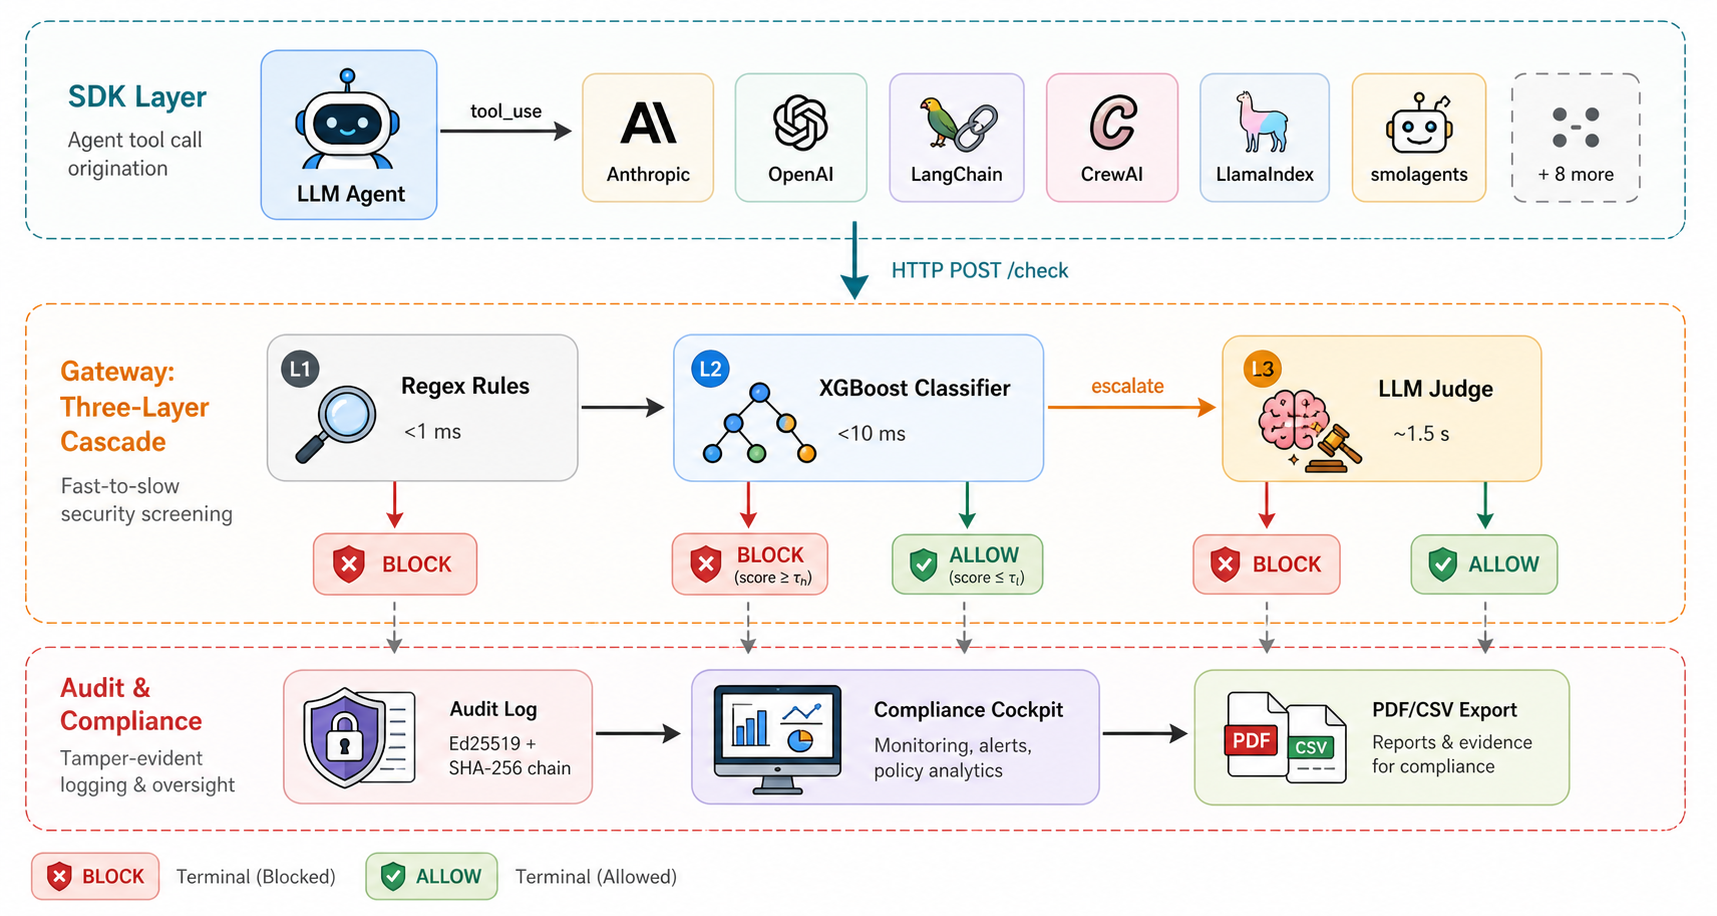
\includegraphics[width=0.93\textwidth]{images/framework.png}
    \vspace{-0.1in}
    \caption{\system architecture overview. The SDK layer instruments 14 agent frameworks to intercept \texttt{tool\_use} calls before execution. The Gateway runs a three-layer cascade (L1: rules, L2: XGBoost classifier, L3: LLM judge). Pending calls route to the Compliance Cockpit for human review. All traces are logged to a tamper-evident audit trail with Ed25519 signatures and SHA-256 hash chaining.}
    \vspace{-0.1in}
    \label{fig:architecture}
\end{figure*}

\section{Introduction}
\label{sec:intro}

Tool-using AI agents~\cite{yao2023react,schick2024toolformer} now routinely issue database queries, shell commands, and API requests---yet evaluating the safety of defenses against malicious tool calls remains an open problem.
Existing benchmarks such as ToolEmu~\cite{ruan2024toolemu}, AgentDojo~\cite{debenedetti2024agentsec}, and InjecAgent~\cite{zhan2024injecagent} have made important progress, but they share a critical blind spot: they test defenses on the \emph{same distribution} the defense was designed for.
A 99\% score on familiar attacks says nothing about the 0\% that may await in production.

We argue that \textbf{honest evaluation requires explicit distribution-shift partitions}.
To make this concrete, we construct \bench, a benchmark of 5{,}525 tool calls from four independent sources, where every record carries a label indicating how far it lies from the defense's training distribution: \emph{in-distribution}, \emph{near-OOD} (same domain, different attack strategy), and \emph{far-OOD} (different domain entirely).
This simple labeling scheme exposes generalization gaps that single-source evaluations conceal---and the gaps are dramatic.

Using \bench, we evaluate 10 defense configurations and present \system, a cost-aware cascade that exploits a key finding from the benchmark: different defense layers fail on \emph{different} inputs, so composing them yields robustness that no single layer achieves.
Our contributions:
\begin{enumerate}[nolistsep,leftmargin=*]
\item \bench, a benchmark with explicit \textbf{distribution-shift partitions} from four independent sources, enabling honest multi-source evaluation of agent safety defenses.
\item A \textbf{comparative evaluation} of 10 defenses revealing that rule-based layers achieve 0\% on OOD attacks and supervised classifiers learn source-specific artifacts (27.2\% OOD block rate)---gaps invisible in single-source evaluation.
\item A \textbf{cost-aware cascade} (rules~$\to$~XGBoost~$\to$~LLM judge) that achieves 99.9\% block rate at 1.1\,ms median latency, demonstrating that complementary failure modes can be composed into robust defense.
\end{enumerate}

\section{Benchmark: \bench}
\label{sec:bench}

\bench aggregates 5{,}525 tool calls (3{,}413 malicious, 2{,}112 benign) from four public sources (Table~\ref{tab:benchcomp}).

\begin{table}[t]
\centering\small
\caption{Composition of \bench by source, label, and distribution partition.}
\vspace{-0.1in}
\label{tab:benchcomp}
\begin{tabular}{lrrrr}
\toprule
Source & Total & Mal. & Ben. & Partition \\
\midrule
InjecAgent~\cite{zhan2024injecagent} & 5{,}304 & 3{,}196 & 2{,}108 & Near-OOD \\
ToolEmu~\cite{ruan2024toolemu} & 144 & 144 & 0 & Near-OOD \\
OWASP~\cite{owasp2025} & 20 & 20 & 0 & Far-OOD \\
AEGIS-self & 57 & 53 & 4 & In-Dist \\
\midrule
\textbf{Total} & \textbf{5{,}525} & \textbf{3{,}413} & \textbf{2{,}112} & \\
\bottomrule
\end{tabular}
\vspace{-0.1in}
\end{table}

\noindent\textbf{Distribution Partitions.}
Each record is tagged relative to the AEGIS L1 rule set:
\emph{In-distribution} records (57) are crafted to match L1 patterns and serve as a ceiling estimate.
\emph{Near-OOD} records (5{,}448) use natural-language prompt injection strategies that bypass syntactic rules.
\emph{Far-OOD} records (20) are OWASP web-security payloads from an entirely different domain.
This partition scheme ensures that a defense cannot inflate its score by overfitting to a single attack distribution.

\section{System: \system Cascade}
\label{sec:arch}

\system is a pre-execution firewall with a three-layer cascade (Figure~\ref{fig:architecture}):

\paragraph{L1: Pattern-Based Rules ($<$1\,ms).}
22 detection patterns across 7 categories (Table~\ref{tab:patterns}) are matched against recursively extracted argument strings.

\paragraph{L2: Supervised Behavioral Classifier ($<$10\,ms).}
Each tool call is encoded into a 15-dimensional feature vector (Table~\ref{tab:features}) capturing argument structure, character-level statistics, and content indicators. A gradient-boosted tree classifier (XGBoost, 300 trees, depth~6) outputs $P(\text{malicious}) \in [0,1]$. Two calibrated thresholds ($\tau_l$, $\tau_h$) control the cascade: confident predictions short-circuit; ambiguous calls escalate to L3. The classifier is pluggable---we also evaluate an unsupervised Isolation Forest~\cite{zhao2019pyod} variant.

\begin{table}[t]
\centering
\footnotesize
\caption{L2 feature vector (15 dimensions).}
\vspace{-0.1in}
\label{tab:features}
\setlength{\tabcolsep}{3pt}
\begin{tabular}{rll}
\toprule
\# & Feature & Description \\
\midrule
1 & arg\_count & Number of top-level arguments \\
2 & total\_arg\_chars & Total character count \\
3 & max\_string\_depth & Deepest nesting level \\
4 & url\_count & URLs in arguments \\
5 & ip\_literal\_count & Raw IP addresses \\
6 & digit\_ratio & Fraction of digit characters \\
7 & uppercase\_ratio & Fraction of uppercase chars \\
8 & punct\_ratio & Fraction of punctuation \\
9 & json\_depth & JSON nesting depth \\
10 & has\_path\_sep & Contains \texttt{/} or \texttt{\textbackslash} \\
11 & has\_curly\_braces & Contains \texttt{\{} or \texttt{\}} \\
12 & shannon\_entropy & Bits per character \\
13 & longest\_run & Longest repeated character run \\
14 & base64\_like & Base64 heuristic score [0,1] \\
15 & hex\_like & Hex string heuristic [0,1] \\
\bottomrule
\end{tabular}
\vspace{-0.15in}
\end{table}

\paragraph{L3: LLM Judge ($\sim$1--2\,s).}
A zero-shot prompt to a frontier model (e.g., Claude Haiku~4.5) classifies the tool call. Only calls in the L2 ambiguous zone reach this layer.

\begin{table}[t]
\centering
\footnotesize
\caption{Detection pattern coverage (22 patterns, 7 categories).}
\vspace{-0.1in}
\label{tab:patterns}
\setlength{\tabcolsep}{2.5pt}
\begin{tabular}{lrl}
\toprule
\textbf{Category} & \textbf{\#} & \textbf{Techniques Covered} \\
\midrule
SQL Injection       & 7 & \makecell[tl]{OR/UNION, blind (pg\_sleep, WAITFOR,\\BENCHMARK, SLEEP), hex, CONCAT, stacked} \\
Path Traversal      & 4 & \makecell[tl]{../, URL-encoded, double-encoded,\\null byte} \\
Shell Injection     & 4 & \makecell[tl]{Metachar, curl/wget+URL,\\\$\{IFS\} splitting, process subst.} \\
Prompt Injection    & 3 & \makecell[tl]{17 sub-patterns: ignore/forget/\\jailbreak/DAN/bypass/roleplay} \\
Sensitive Files     & 2 & \makecell[tl]{14 paths: passwd, shadow, .ssh,\\.aws, .kube, .terraform, .env} \\
Data Exfiltration   & 1 & Payload $>$5KB + external URL \\
PII Leakage         & 1 & \makecell[tl]{11 types: email, SSN, credit card,\\API key, JWT, DB URI, AWS ARN} \\
\bottomrule
\end{tabular}
\vspace{-0.15in}
\end{table}

\section{Evaluation}
\label{sec:eval}

\subsection{Aggregate Performance}

Table~\ref{tab:overall} compares 10 defense configurations spanning four standalone LLM judges, Llama-Guard-3, a keyword blacklist, L1-only rules, and the cascade with two L2 variants and two L3 backends.

\begin{table}[t]
\centering\small
\caption{Headline results on \bench. Block rate is recall on malicious tool calls; FP rate is on benign. Cost is total over the full benchmark (5{,}525 records).}
\vspace{-0.1in}
\label{tab:overall}
\begin{tabular}{lrrrr}
\toprule
Defender & Block\% & FP\% & P50\,ms & \$/run \\
\midrule
\rowcolor{green!8}
\textbf{AEGIS (XGB+Haiku)} & \textbf{99.9} & \textbf{0.09} & \textbf{1.1} & \textbf{0.05} \\
\rowcolor{green!8}
\textbf{AEGIS (XGB+GPT-4o)} & \textbf{99.9} & \textbf{0.09} & \textbf{1.1} & \textbf{0.07} \\
GPT-4o-mini judge & 98.8 & 11.88 & 1204 & 0.36 \\
Haiku~4.5 judge & 96.6 & 0.00 & 2211 & 5.32 \\
GPT-4o judge & 95.7 & 0.00 & 1385 & 0.63 \\
AEGIS (IForest+Haiku) & 94.1 & 0.00 & 2146 & 4.18 \\
Llama-Guard-3 & 67.1 & 0.05 & 73 & 0.00 \\
Keyword blacklist & 2.5 & 0.00 & 0 & 0.00 \\
AEGIS-rules (L1 only) & 1.2 & 0.00 & 1 & 0.00 \\
\bottomrule
\end{tabular}
\vspace{-0.1in}
\end{table}

The XGBoost cascade Pareto-dominates every standalone judge.
But the aggregate numbers tell only part of the story---the per-distribution breakdown is where the benchmark earns its keep.

\subsection{Where Defenses Break: Per-Distribution Analysis}

\begin{table}[t]
\centering\small
\caption{Block rate per distribution partition. $\Delta$ = In-Dist $-$ Far-OOD reveals the generalization gap.}
\vspace{-0.1in}
\label{tab:perdist}
\begin{tabular}{lrrrr}
\toprule
Defender & In-D & Near & Far & $\Delta$ \\
\midrule
GPT-4o-mini judge & 86.8 & 99.0 & 100 & $-$13.2 \\
Haiku~4.5 judge & 77.4 & 96.9 & 100 & $-$22.6 \\
AEGIS cascade & 79.2 & 94.3 & 100 & $-$20.8 \\
Llama-Guard-3 & 56.6 & 67.2 & 80 & $-$23.4 \\
AEGIS-rules (L1) & 77.4 & 0.0 & 0 & +77.4 \\
\bottomrule
\end{tabular}
\vspace{-0.1in}
\end{table}

L1 rules score 77.4\% on in-distribution but \textbf{0\%} on both near-OOD and far-OOD---a $\Delta$ of +77.4 that a single-source evaluation would never reveal.
A benchmark without distribution labels would report the aggregate 1.2\% and conclude the defense is weak; with labels, we see it is \emph{strong on what it knows and blind to everything else}.
LLM judges exhibit the mirror image: negative~$\Delta$ (better on OOD), confirming that semantic reasoning generalizes where pattern matching cannot.
The cascade inherits the best of both regimes.

\subsection{Per-Layer Resolution}

Table~\ref{tab:perlayer} reveals how the cascade exploits the L2 classifier. With supervised XGBoost, L2 resolves 96.3\% of calls at $<$1\,ms, reducing L3 invocations to 1.6\%---a 46$\times$ reduction versus the unsupervised IForest variant.

\begin{table}[t]
\centering\small
\caption{Per-layer resolution: IForest (unsupervised) vs.\ XGBoost (supervised) L2.}
\vspace{-0.1in}
\label{tab:perlayer}
\begin{tabular}{lrrrr}
\toprule
 & \multicolumn{2}{c}{IForest L2} & \multicolumn{2}{c}{XGBoost L2} \\
\cmidrule(lr){2-3}\cmidrule(lr){4-5}
Layer & Calls & \% & Calls & \% \\
\midrule
L1 (rules) & 58 & 1.3 & 58 & 2.1 \\
L2 (classifier) & 268 & 6.0 & 2{,}660 & 96.3 \\
L3 (LLM judge) & 4{,}143 & 92.7 & 45 & 1.6 \\
\bottomrule
\end{tabular}
\vspace{-0.1in}
\end{table}

\subsection{Cross-Source Generalization}

If a supervised classifier resolves 96\% of traffic, a natural worry is that it has memorized the training distribution.
Table~\ref{tab:xsource} confirms this concern: XGBoost trained on InjecAgent alone drops to 27.2\% when tested on ToolEmu+OWASP+Self.
The asymmetry is informative---training on the smaller but more diverse set yields 89.4\% on InjecAgent---suggesting source diversity matters more than source size.
This is precisely why the cascade needs its L3 backstop, and why benchmarks need multi-source evaluation.

\begin{table}[t]
\centering\small
\caption{Cross-source generalization of XGBoost L2 (no L3). Block rate drops on OOD sources, validating the need for multi-source evaluation.}
\vspace{-0.1in}
\label{tab:xsource}
\begin{tabular}{llrr}
\toprule
Train source & Test source & Block\% & FP\% \\
\midrule
InjecAgent & InjecAgent (held-out) & 93.4 & 0.00 \\
InjecAgent & ToolEmu+OWASP+Self & 27.2 & 0.00 \\
ToolEmu+OWASP+Self & InjecAgent & 89.4 & 0.00 \\
\bottomrule
\end{tabular}
\vspace{-0.1in}
\end{table}

\subsection{Adaptive Robustness}

We evaluate robustness against an LLM-driven red-team attacker (Claude Sonnet~4.6) that iteratively rewrites malicious tool calls over 5~rounds to bypass each defender (Figure~\ref{fig:adaptive}).
On 53~seed attacks: the keyword blacklist reaches 97\% cumulative bypass by round~4, AEGIS rules 74\%, and the LLM judge 89\%.
The cascade benefits from complementary failure modes: attacks that bypass rules often fail on the LLM judge and vice versa.

\subsection{Obfuscation Robustness}

We evaluate the L1+L2 cascade (no L3) on 32{,}829 attacks generated by 9 obfuscation transforms, \emph{training only on clean data}.
Block rate remains $\ge$97.5\% with 0\% FP across all transforms (Figure~\ref{fig:obfuscation}).
This zero-shot robustness validates the L2 feature design: structural features like \texttt{total\_arg\_chars} and \texttt{shannon\_entropy} are invariant to surface-level transformations.

\section{Related Work}
\label{sec:related}

\paragraph{Agent Safety Benchmarks.}
ToolEmu~\cite{ruan2024toolemu}, AgentDojo~\cite{debenedetti2024agentsec}, and InjecAgent~\cite{zhan2024injecagent} provide valuable attack corpora but evaluate defenses on a single source distribution.
\bench reuses their data while adding explicit OOD partitions that reveal generalization failures invisible in the original evaluations.

\paragraph{Trustworthiness and Guardrails.}
TrustLLM~\cite{huang2024position} and TrustEval~\cite{wang2024trusteval} assess trust at the model output level; \system operates one layer downstream on agent \emph{actions}.
Llama Guard~\cite{inan2023llama} classifies text-level safety; Langfuse~\cite{langfuse2024}, Helicone~\cite{helicone2024}, and Arize~\cite{arize2024} trace agent behavior post-execution.
\system differs in scope (structured tool calls) and timing (pre-execution), and adds a cost-aware cascade absent from existing guardrail systems.

\section{Conclusion}

The central lesson of this work is that \emph{distribution-shift labels change what benchmarks can teach us}.
Without them, a 22-rule scanner appears weak (1.2\% aggregate) and an LLM judge appears strong (96.6\%); with them, we see that the scanner is a Maginot Line (77\% in-distribution, 0\% OOD) and the judge generalizes well but at 1{,}000$\times$ the cost.
The cascade exploits complementary failure modes---cheap layers handle the familiar, the judge backstops the novel---achieving 99.9\% block rate at 1.1\,ms while remaining above 97.5\% under obfuscation transforms it was never trained on.
We hope the distribution-shift labeling scheme in \bench will inform how future agent safety benchmarks are constructed.
The benchmark, evaluation framework, and defense system are available under the MIT license.

\clearpage
\bibliographystyle{ACM-Reference-Format}
\bibliography{references}

%%%%%%%%%%%%%%%%%%%%%%%%%%%%%%%%%%%%%%%%%%%%%%%%%%%%%%%%%%%%
%%                      APPENDIX                          %%
%%%%%%%%%%%%%%%%%%%%%%%%%%%%%%%%%%%%%%%%%%%%%%%%%%%%%%%%%%%%
\clearpage
\appendix

\section{Feature Importance}
\label{app:feature_importance}

Figure~\ref{fig:feature_importance} shows XGBoost L2 gain-based feature importances.
\texttt{total\_arg\_chars} dominates at 76.3\%, reflecting that malicious tool calls carry longer argument strings.

\begin{figure}[h]
    \centering
    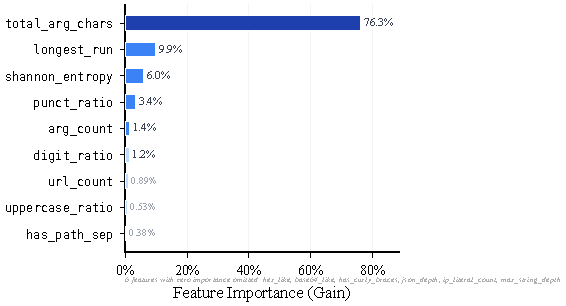
\includegraphics[width=\columnwidth]{images/feature_importance.pdf}
    \caption{XGBoost L2 feature importance (gain).}
    \label{fig:feature_importance}
\end{figure}

\section{Obfuscation Robustness}
\label{app:obfuscation}

We test the XGBoost cascade (L1+L2, no L3) on 32{,}829 obfuscated attacks from 9 transforms, trained only on clean data (zero-shot).
Block rate stays $\ge$97.5\% with 0\% FP (Figure~\ref{fig:obfuscation}).

\begin{figure}[h]
    \centering
    
\includegraphics[width=\columnwidth]{images/obfuscation_robustness.pdf}
    \caption{Block rate on 9 obfuscation transforms (zero-shot).}
    \label{fig:obfuscation}
\end{figure}

\section{Obfuscation Robustness}
\label{app:obfuscation}

\begin{figure}[h]
    \centering
    
\includegraphics[width=\columnwidth]{images/obfuscation_robustness.pdf}
    \caption{Block rate on 9 obfuscation transforms (zero-shot, trained on clean data only). All transforms maintain 0\% FP.}
    \label{fig:obfuscation}
\end{figure}

\section{Threshold Sensitivity}
\label{app:threshold}

\begin{figure}[h]
    \centering
    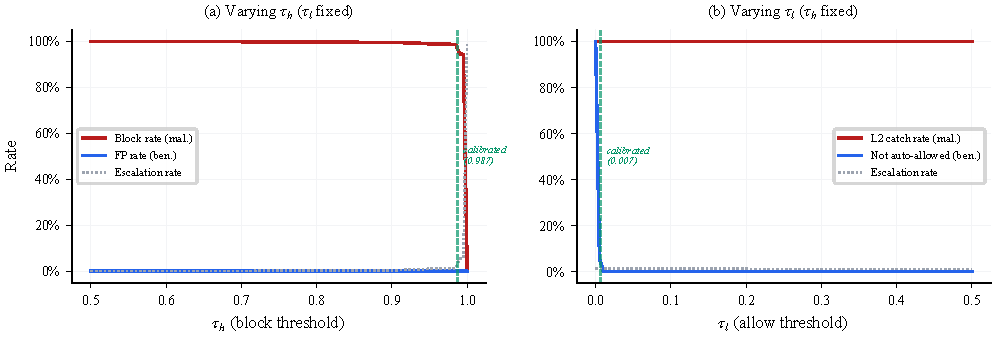
\includegraphics[width=\columnwidth]{images/threshold_sensitivity.pdf}
    \caption{Threshold sensitivity: calibrated values sit in flat regions, indicating robustness to perturbation.}
    \label{fig:threshold}
\end{figure}

\section{Adaptive Red-Team}
\label{app:adaptive}

\begin{figure}[h]
    \centering
    
\includegraphics[width=\columnwidth]{images/adaptive_redteam.pdf}
    \caption{Cumulative bypass rate over 5 adversarial rounds (53 seeds, Claude Sonnet~4.6 attacker).}
    \label{fig:adaptive}
\end{figure}

\end{document}
